\documentclass[
  journal=largetwo,
  year=2023,
]{cup-journal}

\usepackage{amsmath}
\usepackage[nopatch]{microtype}
\usepackage{booktabs}
\usepackage[]{hyperref}
\usepackage{physics}


\title{Physical Implementation of Quantum Computers}

\author{Thiago Mattos}
\affiliation{Universidade Federal de Minas Gerais, Departamento de Física, Belo Horizonte, 31270-901, Minas Gerais, Brazil}
\email[T. Mattos]{thiagomattos@ufmg.br}

\author{Eric Botelho}
\affiliation{Universidade Federal de Minas Gerais, Departamento de Física, Belo Horizonte, 31270-901, Minas Gerais, Brazil}

\addbibresource{references.bib}

\keywords{quantum computer, superconducting qubits, ion trap, photonic model}

\begin{document}

\begin{abstract}
  This work aims to explain the physical principles of quantum computers. We will discuss how some physical systems can be used to peform computation, specialy with respect to three chosen impleentations, as well as the main advantages and disadvantages of each implementation.
  The implementations we will discuss are ion traps, photonic models and solid state systems. The ion trap model is based on the manipulation of ions in a trap, the photonic model is based on the manipulation of photons in a cavity and the solid state model is based on the manipulation of electrons in a superconducting circuit. The main advantages and disadvantages of each model are presented, as well as the main challenges for the construction of a quantum computer.

\end{abstract}

\section{Introduction}

When delving into the realm of quantum computing, a crucial inquiry arises: Can a quantum computer truly be realized in the physical world? This article is devoted to the exploration and elucidation of the feasibility of physically implementing quantum computers. It aims to present various models of quantum computers while engaging in a concise discussion and general analysis of the subject matter.

To grasp why the physical realization of a quantum computer is viable, it is imperative to emphasize the primary obstacle in its construction: decoherence. Decoherence can be perceived as the transformation of quantum information into classical information, thereby constituting the principal barrier that separates the two domains. One might ponder why classical mechanics becomes apparent at larger scales when, in theory, the macroscopic outcomes should be explained as the culmination of multiple microscopic effects. Well, classical mechanics can be comprehended as a specific case within the vast framework of quantum mechanics, characterized by profound decoherence and the complete loss of ``quantum'' information. But why does this happen? Decoherence materializes due to the interaction between a quantum system and its surroundings, favoring certain states while obliterating superpositions.

\section{Physical Propertires}

Knowing all the obstacles of quantum systems in real situations, DiVicenzo discussed in his article \autocite{divincenzo_2000_the} the requirements for the existence and creation of a quantum computer, establishing the following criteria:
\begin{enumerate}
  \item \emph{A scalable physical system with well characterized qubits}
  \item \emph{The ability to initialize the state of the qubits to a simple fiducial state as \(\ket{000\dots}\)}
  \item \emph{Long relevant decoherence times, much longer than the gate operation time}
  \item \emph{A “universal” set of quantum gates}
  \item \emph{A qubit-specific measurement capability}
  \item \emph{The ability to interconvert stationary and flying qubits}
  \item \emph{The ability faithfully to transmit flying qubits between specified locations}
\end{enumerate}

Before going into detail about the physical implementation of quantum computers, let's establish some definitions regarding physical systems.


The Decoherence time of a quantum system is the time it takes to interact with it's environment and turn this pure state like \(\ket{\psi} = a\ket{0} + b\ket{1}\) into a mixture \( \rho = |a|^2\ketbra{0}{0} + |b|^2\ketbra{1}{1} \).

The Gate Operation Time is the duration required to perform the given unitary transformation.


So now let's summarize some prerequisites to do some reliable quantum computation in real quantum states. First of all, the first requirement tells us that we need a scalable physical system with well characterized qubits, otherwise means that we need some quantum two-level system to form our computational basis \(\ket{0}\) and \(\ket{1}\), some examples of real quantum systems that can represent a qubit are the vertical and horizontal polarization of a single photon, the two states of a spin 1/2 particle traditionally labeled as spin up and spin down, the two hyperfine levels of the ground state of the neutral hydrogen atom. Furthermore, when we call some qubit system well characterized we mean that we must know the internal Hamiltonian which is related to the total energy associated with the system and tell us how this system evolves over the time through the Schrödinger's equation:

\begin{equation}
  \begin{aligned}\label{eq:1}
    i\hbar\frac{\partial \ket{\psi}}{\partial t} = \hat{H}\ket{\psi}
  \end{aligned}
\end{equation}

So if we consider the trivial case where the eigenstates of \(\ket{\psi}\) are also eigenstates of the Hamiltonian operator (which in this case don't fluctuate over time), we can write the state like \(\ket{\psi(t)} = \sum{\alpha_i(t)\ket{i}}\) and therefore considering \(\lambda_i\) the eigenvalues of \(\hat{H}\)  by the Schrodinger equation we have \(\sum{(\alpha_i(t)\lambda_i - i\hbar\frac{d\alpha_i(t)}{dt})\ket{i}} = 0\), solving the differential equation we finally get:

\begin{equation}
  \begin{aligned}\label{eq:2}
    \alpha_i(t) = \alpha_i(0)e^{-\frac{i\lambda_i t}{\hbar}}
  \end{aligned}
\end{equation}

Knowing that quantum gates are simply unitary transformations, to have a universal set of quantum gates using real quantum systems we need to build some unitarys like \(U_1 = e^{\frac{iH_1t}{\hbar}}, U_2 = e^{\frac{iH_2t}{\hbar}}\). So to perform some sequence of transformations the quantum computer need to ``turn on'' \(H_1\) from 0 to t and then turn off \(H_1\) and turn on \(H_2\) from t to 2t.
Inside a classical computer the state of a bit is defined by a pulse signal of a square wave, it is basically a boolean signal of whether current is flowing or not. An example is: if the signal is 5V represent it as bit 1, if it is 0V represent it as bit 0, these signals are updated according to the ``clock time'' of the computer, given by the frequency of the processor. When we go to the quantum world things change of situation, now it is no longer a control variable like a pulse, quantum states have assertive time evolution and therefore can't be idle for a long time before executing an operation. The only way to generate multiple states when we need like we did in classical computers is to turn on and off the interaction smoothly and slowly enough that an adiabatic approximation is accurate. Out of that, quantum gates have errors inherent to their implementations, be them systematic or random, but fortunately it have be shown that if the decoherence time of the quantum system that represents a qubit is \(10^4\) - \(10^5\) times the ``clock time'' of the quantum computer some error correction code can succeed in return the required state with great fidelity. Basically, what error correction tries to do is to identify everything that is the result of errors in a subspace orthogonal to the subspace of the ``code'' but all this has a price, and as John Preskill argues in his article ``Reliable Quantum Computers'' outlining some laws for fault-tolerant computation, we can't use the same qubit twice to handle the error, after all if there was an error in this handling it would propagate indefinitely, so for each qubit used in the operations, we would have to have an ancillary. Also he claims some criterias to fault-tolerant computation, they are:\\

\begin{enumerate}
  \item \emph{Don't use the same bit twice}
  \item \emph{The ancilla must be prepared properly, so that the fault-tolerant syndrome
          measurement diagnoses the errors without spoiling the coherence of the data}
  \item \emph{Copy the
          errors, not the data}
  \item \emph{Verify when you encode a known quantum state}
  \item \emph{Repeat operations}
  \item \emph{Use the right code}
\end{enumerate}

Furthermore, the measurement capability of a qubit can be ;``demolition'' or ``non-demolition'' depending if the measurement changes the quantum state or not, but does not change the state of neighboring qubits, even if they perform operations in parallel.

The Hamiltonian, from classical mechanics, is the function that represents the total energy of a system, which is usually its kinetic energy plus its potential energy. In quantum mechanics, the hamiltonian is the Hermitian operator(as we know these matrices have real eigenvalues) that determines the time evolution of the system and whose eigenvalues correspond to the possible energy levels of the same.
It is important to note that the possibility of a quantum system assuming only discrete values of energy by quantum mechanics does not imply that the number of energies is finite. Indeed, the discrete or continuous nature of the energy spectrum depends on the specific properties of the system under consideration.

There are quantum systems that have a discrete energy spectrum, which means that there are only certain allowable values of energy that the system can have. A classic example is the quantum harmonic oscillator, in which energy is quantized in integer multiples of a specific quantity, known as energy quantum. In this case, the energy spectrum is discrete but infinite, as there are infinitely many allowed values of energy, in other words, this means that the Hamiltonian will not necessarily have a finite number of eigenstates, after all, the quantum states are found in Hilbert space, which in turn is an infinite complex vector space with inner product. For the case of a measure of infinite and non-degenerate eigenstates, according to the 4th postulate of quantum mechanics, the probability of obtaining values between x and x+dx is given by: \(dP(x) = |\braket{x}{\psi}|^{2}dx\). The Hamiltonian is usually written as:

\begin{equation}
  \begin{aligned}\label{eq:3}
    H(p, x) = \frac{p^2}{2m} + V(x)
  \end{aligned}
\end{equation}

When we transfer the notions to quantum mechanics we are no longer dealing with scalars, but with the operators referring to each magnitude, usually in the case of the Hamiltonian, in terms of momentum and position. So the Hamiltonian operator would be:

\begin{equation}
  \begin{aligned}\label{eq:4}
    \hat{H}(\hat{p}, \hat{x}) = \frac{\hat{p}^2}{2m} + V(\hat{x})
  \end{aligned}
\end{equation}

Now, let's use Schrodinger's equation and the equation above to obtain a literal expression that takes into account the quantization of magnitudes and that now the Hamiltonian is an operator. So we have: \(i\hbar\frac{\partial \ket{\psi}}{\partial t} = \frac{\hat{p}^2}{2m} + V(\hat{x})\ket{\psi}\), now let's discretize the operation and determine the result of the momentum and position operators acting on the wave function. \(\psi(x) = \bra{x}\ket{\psi}\) and then \(\hat{x}\psi(x) = \bra{x}\hat{x}\ket{\psi}\). With \(\hat{x}\ket{\psi} = \int{\bra{x}\hat{x}\psi(x^{'})\ket{x^{'}}dx^{'}}\) Finally resulting in:

\begin{equation}
  \begin{aligned}\label{eq:5}
    \hat{x}\psi(x) = x\psi(x) = x\braket{x}{\psi}
  \end{aligned}
\end{equation}

Now applying the same reasoning to the momentum operator \(\hat{p}\psi(x) = \bra{x}\hat{p}\ket{\psi}\) how we know \(\braket{p}{x} = \frac{e^{\frac{-ipx}{\hbar}}}{\sqrt{2\pi}}\) \(\hat{p}\psi(x) = \int{\psi(p)\bra{x}\hat{p}\ket{p}dp}\)
\(\hat{p}\ket{p} = p\ket{p}\). Finally resulting in:

\begin{equation}
  \begin{aligned}\label{eq:6}
    \hat{p}\psi(x) = -i\hbar\frac{\partial\psi(x)}{\partial x}
  \end{aligned}
\end{equation}

Putting these results into the Schrodinger equation we get:

\begin{equation}
  \begin{aligned}\label{eq:7}
    \frac{-\hbar^{2}}{2m}\frac{\partial^{2}\psi}{\partial x^{2}} + V(x)\psi = i\hbar\frac{\partial \psi}{\partial t}
  \end{aligned}
\end{equation}

Moving on for a more practical example, let's consider that the system that represents our qubits are the two states of a spin 1/2 produced of an electron produced by a magnetic field in the z direction, the states \(\ket{\uparrow}\) and \(\ket{\downarrow}\), considering the results of the Stern-Gerlach experiment, we know that we can receive \(+\frac{\hbar}{2}\)  either \(-\frac{\hbar}{2}\) as result of measurement. The first step is to determine the total energy of the system, which in this case will be given by the directional energy of the magnetic field in the \(\hat{z}\) direction. So to begin with, let's deduce the classical case and then perform the first quantization. The first quantization is based on the transformation of a model or theory of classical mechanics to the equivalent in quantum mechanics and basically consists of passing the magnitudes involved to Hermitian operators, respecting the commutation between them.\\
So the angular momentum of a eletron in orbit is given by \(\Vec{L} = mvR\hat{z}\)  the magnetic moment is \(\vec{M} = IA\hat{z}\)  which is equal to \(\vec{M} = (\frac{qv}{2\pi R}\pi R^{2})\hat{z} = \frac{qmvR}{2m}\hat{z} = \frac{q}{2m}\Vec{L}\) . Therefore the total energy of the system (and hamiltonian function) is given by classical mechanics is given by:

\begin{equation}
  \begin{aligned}\label{eq:8}
    U = -\Vec{M}\cdot\vec{B}
  \end{aligned}
\end{equation}

\section{Photonic Model}

\section{Ion Trap}
The study of atomic structure and its associated energy levels provides great insight into fundamental quantum properties that can be harnessed to realize actual qubits.

\subsection{Apparatus Description}

To harness the quantum effects of a charged atom and enable precise control over its quantum states, it is essential to decouple the atom from any external influences. This necessitates the development of a method to confine the ion within a vacuum environment. One widely utilized approach involves the use of an electromagnetic field source to immobilize the charged particle. However, the utilization of a static electric field that can trap the particle in all directions is prohibited by Earnshaw's theorem \autocite{jones_1980_earnshaws}.

Nevertheless, there exists a viable solution that enables the confinement of the charged particle in space. By employing time-varying electrical fields, it becomes possible to generate an average force that restricts the ion's movement. This ingenious type of trap is referred to as a Paul trap \autocite{paul_1953_notizen}. At its core, a Paul trap consists of a set of electrodes capable of producing a quadrupolar electric field. This field configuration facilitates the trapping of the charged particle by exerting forces that counteract its tendency to escape along certain axes while allowing its confinement within others.

The fundamental principle underlying the operation of a Paul trap relies on the interplay between the electric fields generated by the electrodes and the motion of the charged ion. As the ion moves within the trap, its interaction with the oscillating electric fields causes it to experience a restoring force towards the trap's center. This confinement allows for stable trapping and manipulation of the ion's quantum states, which provides a good foundation for the development of a quantum computer.

There are usualy two types of Paul traps configuration, one with layout of quadrupolar electrodes that traps the ion in add three dimensions (point traps), and one with two RF trapping plus and a static eletric field that traps the ion in a plane (linear traps).
The point traps have only one point where the field is zero, thefore for multiple ions to be trapped in the same trap they need to be cooled to a point where they are almost still, or it leads to lost of fidelity.
Linear traps in general have a line where the field is zero, therefore it is possible to trap multiple ions in the same trap, and trought variation on the static field, ions can be moved and rearranged in the trap.



\begin{figure*}
  \centering
  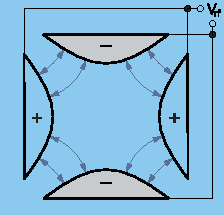
\includegraphics[height=4cm]{figs/fig1/g96736.pdf}
  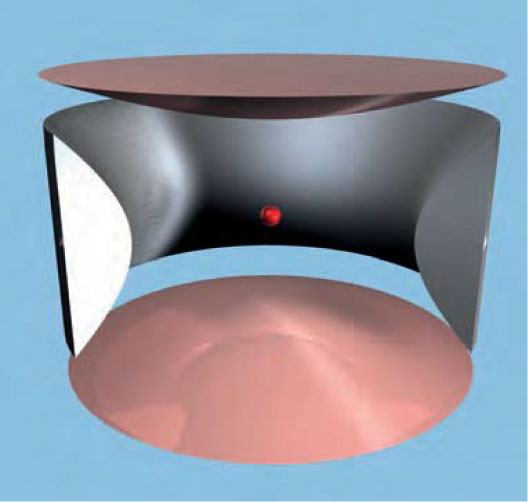
\includegraphics[height=4cm]{figs/fig1/p5_6.png}
  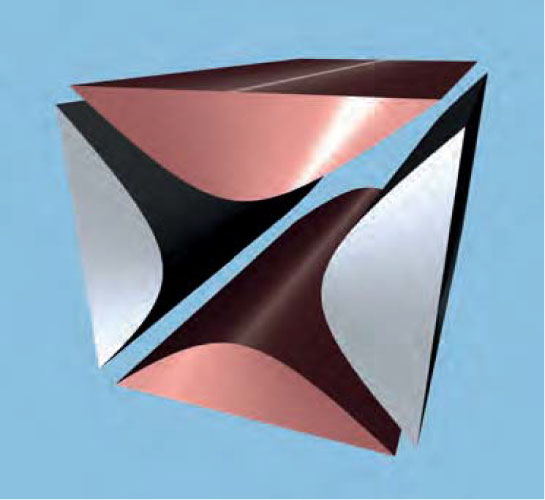
\includegraphics[height=4cm]{figs/fig1/p5_5.png}
  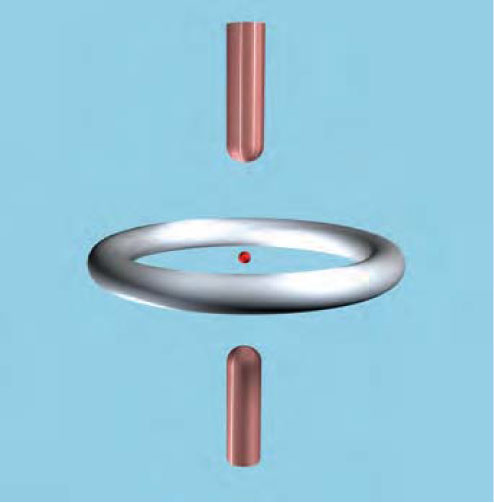
\includegraphics[height=4cm]{figs/fig1/p5_4.png}

  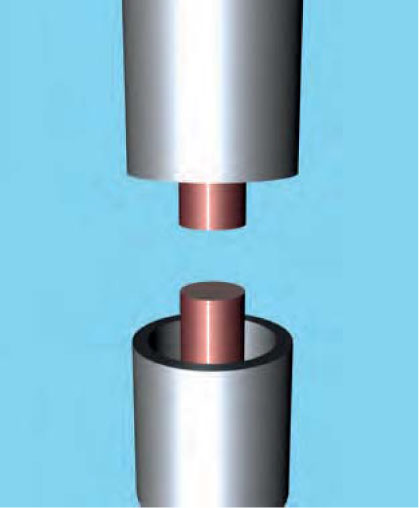
\includegraphics[height=4cm]{figs/fig1/p5_7.png}
  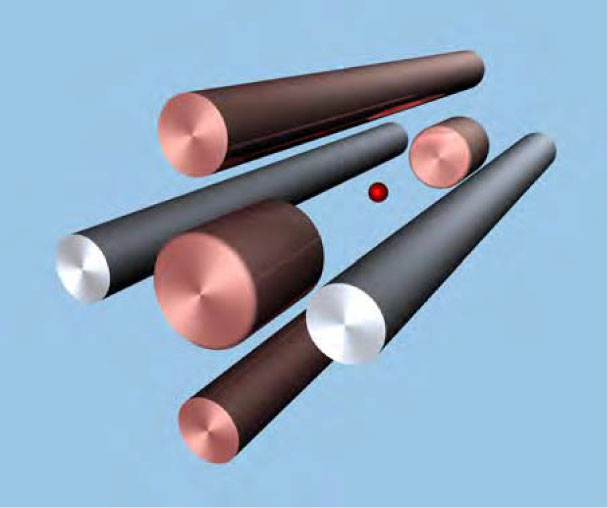
\includegraphics[height=4cm]{figs/fig1/p5_1.png}
  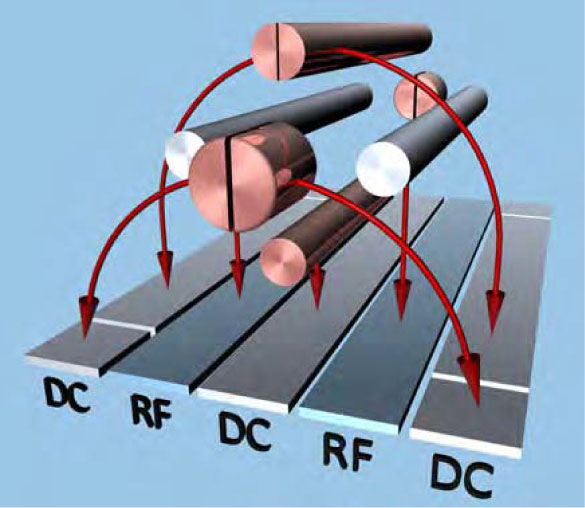
\includegraphics[height=4cm]{figs/fig1/p5_2.png}
  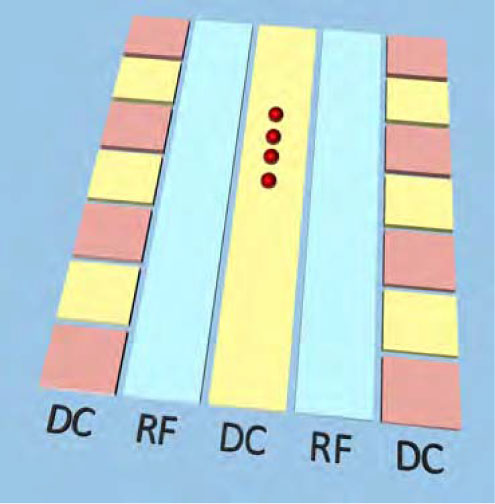
\includegraphics[height=4cm]{figs/fig1/p5_3.png}

  \caption{(Reproduced from \autocite{brownnutt_2015_iontrap}) (a) The fundamental concept of RF trapping involves the generation of quadrupolar fields that oscillate at an RF frequency. This is achieved by employing a set of (parabolic) electrodes. (b) The simplest version of the basic RF trap exhibits cylindrical symmetry and is known as the ``ring and endcap'' point-trap configuration. (c) Another simple variation of the RF trap is the translationally symmetric design, which forms a quadrupole mass filter and can be utilized as a linear trap. (d,e) Additional configurations that share the same topology as the geometry shown in (b) but exhibit slight deformations. (f) Similar topologically equivalent deformations can be applied to the geometry shown in (c), where extra endcap electrodes are incorporated to create a four-rod, linear trap. (g) By manipulating the four-rod trap in (f), it is possible to arrange all the electrodes in a single plane, resulting in a linear ``surface-electrode trap.'' (h) In a linear trap, a subset of the electrodes (depicted here using a surface-electrode trap, but applicable to other linear trap geometries as well, such as the one shown in (f)) can be segmented to enable trapping in multiple zones along the axial direction.}
\end{figure*}


\section{Solid State: Superconducting Qubits}

\section{Comparative Analysis}

\section{Conclusion}

\printendnotes

\printbibliography

\appendix

\section{Example Appendix Section}

Lorem ipsum dolor sit amet, consectetur adipiscing elit, sed do eiusmod tempor incididunt ut labore et dolore magna aliqua. Lorem ipsum dolor sit amet, consectetur adipiscing elit, sed do eiusmod tempor incididunt ut labore et dolore magna aliqua. Lorem ipsum dolor sit amet, consectetur adipiscing elit, sed do eiusmod tempor incididunt ut labore et dolore magna aliqua.

\end{document}